%\documentclass[review]{cvpr}
\documentclass[final]{cvpr}

\usepackage{times}
\usepackage{epsfig}
\usepackage{graphicx}
\usepackage{amsmath}
\usepackage{amssymb}

% Include other packages here, before hyperref.

% If you comment hyperref and then uncomment it, you should delete
% egpaper.aux before re-running latex.  (Or just hit 'q' on the first latex
% run, let it finish, and you should be clear).
\usepackage[pagebackref=true,breaklinks=true,colorlinks,bookmarks=false]{hyperref}


\def\cvprPaperID{15463} % *** Enter the CVPR Paper ID here
\def\confYear{CVPR 2022}
%\setcounter{page}{4321} % For final version only

\author{Lingxi Zhang
\\ Carnegie Mellon University
\\ Pittsburgh, Pennsylvania 15213
\\ {\tt\small lingxiz@andrew.cmu.edu}
% For a paper whose authors are all at the same institution,
% omit the following lines up until the closing ``}''.
% Additional authors and addresses can be added with ``\and'',
% just like the second author.
% To save space, use either the email address or home page, not both
}

%%%%%%%%% TITLE
\title{Effect of Various Parameters in Flash Cut Foreground Extraction with Flash/Non-Flash Pairs}


\begin{document}

\maketitle


%%%%%%%%% ABSTRACT
\begin{abstract}
   This paper presents a partial implementation of the previous 
   \textbf{flash cut foreground extraction with flash and no-flash image pairs} 
   algorithm \cite{Authors1}. It only used the most essential foreground energy
   and background energy term to compute the labeling due to time and scope 
   complexity of the original project. It also uses different methods of 
   mean and standard deviation estimation to compute the probability attributes. 
   This paper aims to discuss the effect of various parameters on final foreground 
   extraction results, and as a side result, whether we can implement continuous distinction 
   rather than binary distinction.

\end{abstract}

%%%%%%%%% BODY TEXT
\section{Introduction}

Image segmentation, which is the process of partitioning a digital image into multiple 
image segments, is one of the most important problems in the world of 
computer vision. Nevertheless, generating quality segmentation result
from limited sources of images are still challenging. Many methods rely 
heavily on simply more images or additional information, such as motions, 
stereo, and infrared light, or the assumption of a static background.
In a lot of situation, these factors are either costly to get and compute, 
or just impossible to obtain in some cases. 

Luckily, we already have a 
well-established method from \textit{Sun et al.} that use no additional factors 
other than the images themselves and only use two shots of images : the flash
one and the non-flash one. Additionally, their method does not even require 
static setting of the background and the object. Relative small movement of the scene 
is fine instead of absolutely static scene.
%------------------------------------------------------------------------
\section{Background}

Existing foreground extraction framework only works when the foreground in
the pictures is very far away from the background so that the flash effect is very
different between foreground and background(essentially a binary distinction).
However, in some cases the foreground is not so far from the background. As a
result, the flash still has some influence over the part with deeper depth instead
of zero influence in the previous assumption. As a result, the definition of
background and foreground is not as clear as before. The question is, is there 
anyway that we can decice how much stuff will be in the background and foreground?

There are indeed some practical applications of this in real life. For instance, if Bob
stands in front of Lincoln’s statue(which is partially affected by the flash), and
there are many skyscrapers in the far end. Traditional foreground extraction
may only include Bob in the picture. But if we relax our distinction in the standard
algorithm to some extent, we can also include Lincoln’s statue. 

\section{Problem Formulation}
A foreground/background segmentation can be formulated as a binary labeling problem.
The answer of the problem are simply labels of 0(background) or 1(foreground) for all 
pixels in the images. 

Let us denote the flash image $I^f$, the no-flash image $I^n$, the labeling for pixel $p$
is $x_p \in \{0,1\}$. The foreground layer is extracted by minimizing the following energy of 
an Markov Random Field(MRF):
\begin{align}
   E(X) = \sum_{p} E_d(x_p) + \alpha \sum_{p,q}E_s(x_p,x_q)
\end{align}
where $E_d(x_p)$ is the data term for each pixel $p$, and $E_s(x_p,x_q)$ is the 
smoothness term associated with two adjacent pixels $p$ and $q$. It is called 
"smoothness" because we penalize different labeling of adjacent pixels that 
have small intensity difference in the original image. For the sake of this project,
we ignore this term and only focus on the data term as in that case the local optimal 
answer is also the global optimal answer, saving us from solving complex equations with 
gradient descent or other complex methods.

The original data term $E_d(x_p)$ models the flash effects on the
foreground, the (motion compensated) background, and the
color likelihood. It consists of three terms:
\begin{align}
   E_d(x_p) = \gamma_fE_f(x_p) + \gamma_fE_f(x_p) + E_c(x_p)
\end{align}

Again for the sake of complexity we emit the color term as well and focus on the first two 
terms.

\subsection{The foreground term $E_f$}
$E_f$ is the foreground flash term, which tends to label
the pixel with significant appearance change as foreground.

In the original paper, color histograms are used for the computation. We will use 
grayscale intensity histograms that simplifies the process.

Basically, the histogram is just made of a number of evenly-distributed bins. 
Each bin holds the count of pixels in the original image that has the intensity 
inside the range of the bin. Since in our experiment the image is large enough to 
provide efficient sources of bin elements, we will just use 256 bins for a 8-bit image,
which means each pin will hold pixels that have a single intensity value.

Let us denote the corresponding bin for pixel $p$ is $k_p$, and $h_k$ is the count of 
pixels in bin $k$. Then the flash ratio for the flash and non-flash images is defined as
\begin{align}
   r_p^f = \max\{\frac{h_{k_p}^f - h_{k_p}^n}{h_{k_p}^f}, 0\}, 
   r_p^n = \max\{\frac{h_{k_p}^n - h_{k_p}^f}{h_{k_p}^n}, 0\}
\end{align} 

In other words, the flash ratio refers to how much positive change in pixel count from 
the flash classification to the non-flash classification for a single pixel $p$ and 
vice versa. If the flash ratio is high, that means the pixel is more likely to belong 
to the foreground since the flash has more effect on the foreground. 

We then define the energy term based on the flash ratio with a robust parameter $\delta$ as
\begin{align}
   E_f(x_p) = 
   \left\{\begin{matrix}
      0 & x_p = 0 \\
      \frac{1}{1-\delta}(\max\{r_p,\delta\} - \delta) & x_p = 1 \\
     \end{matrix}
     \right.
\end{align}
In our experiment we set the value of $\delta$ to 0.2.

\subsection{The background term}
$E_m$ is the background flash term, which models the
motion-compensated flash effect on the background. It
tends to label the pixel with good matching and small
appearance changes as background. This energy term
considers both flash and motion cues. 

Suppose we have a dense motion field $m = \{m(p)\}$, such that 
$p' = m(p)$ is simply the corresponding pixel in the flash image
(after considering motion movement) compared to the original no-flash image.
Since the image difference $I_d$ is defined as 
\begin{align}
   I_d = I_{p'}^f - I_{p}^n
\end{align} 

Since the user is expected to capture the flash/no-flash images
with distant background in quick succession, the appearance
change of the background is expected to be small
and uniform. It is thus reasonable to model the flash difference
distribution of all background pixels as a \textbf{Gaussian
distribution} $N(I_d|\mu, \sigma^2)$. Then, we can define the 
probability of a pixel $p$ belonging to the background as 
\begin{align}
   p_b(x) = \exp(-\sigma_b(I_d - \mu)^2)
\end{align}
where $\sigma_b$ is the adjust standard deviation value so that the 
pixel with flash difference within the $\pm 3\sigma$ interal will be given
a higher probability to be background. Finally, we can define the energy term 
as 
\begin{align}
   E_m(x_p) = 
   \left\{\begin{matrix}
      2\max\{p_b(x_p),0.5\} - 1 & x_p = 1 \\
      0 & x_p = 0 \\
     \end{matrix}
     \right.
\end{align}
with this definition, $E_m(x_p)$ is normalized to be in the range $[0,1]$. 

\subsection{Mean and Standard Deviation Estimation for the Background Probability}
We use a different method from the original paper to estimate $\mu $ and $\sigma$. 
The original paper suggests a combination of making 1D histogram of flash difference 
and use a SIFT sparse feature matching to estimate the $\mu $ and $\sigma$ more accurately.
I simply calculate the mean from the distribution directly, and leave the standard deviation
$\sigma$ actually a tunnable variable in later experiments. (In the original paper they 
use the first local min bin after the mean and cutting off values of threshold to estimate 
the standard deviation). 

The default setting for the $\sigma$ value is 0.10.

\subsection{Motion Estimation}
We use the dense optical flow computation method from \cite{Authors2} and 
simply call \textit{cv2.calcOpticalFlowFarneback()} from python opencv library.

Basically we compute a 2D flow vector $flow = \{(dx,dy)\}$ for each pixel such 
that  
\begin{align}
   I_f(x,y) = I_n(x+dx,y+dy)
\end{align}

For more details please refer to the paper.

\section{Methodlogy}
We took pictures around 4-5 pm at my backyard with tripod and Nikon D3500 camera.
Notice during the shots there are some non-ignorable movements of both camera 
and the scene object.


\begin{figure}[ht]
   \centering
   \includegraphics[scale=0.15]{../data/input/arthas_i.JPG}
   \includegraphics[scale=0.15]{../data/input/arthas_f.JPG}
   \caption{Original flash and no-flash pairs}
\end{figure}
 
\section{Results}

\begin{figure}[ht]
   \centering
   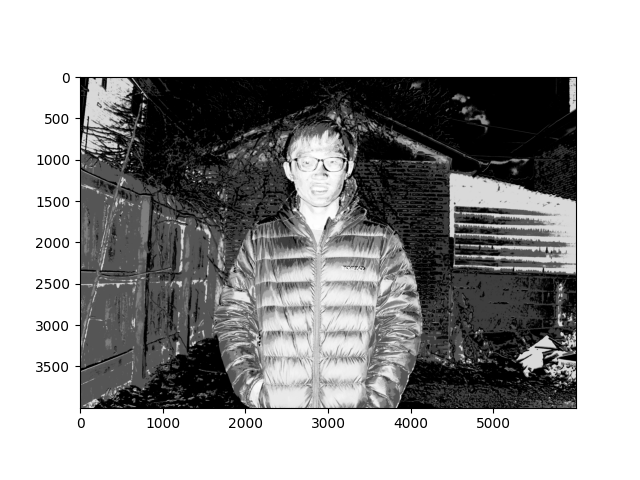
\includegraphics[scale=0.035]{../data/output/arthas_nf_ratio.png}
   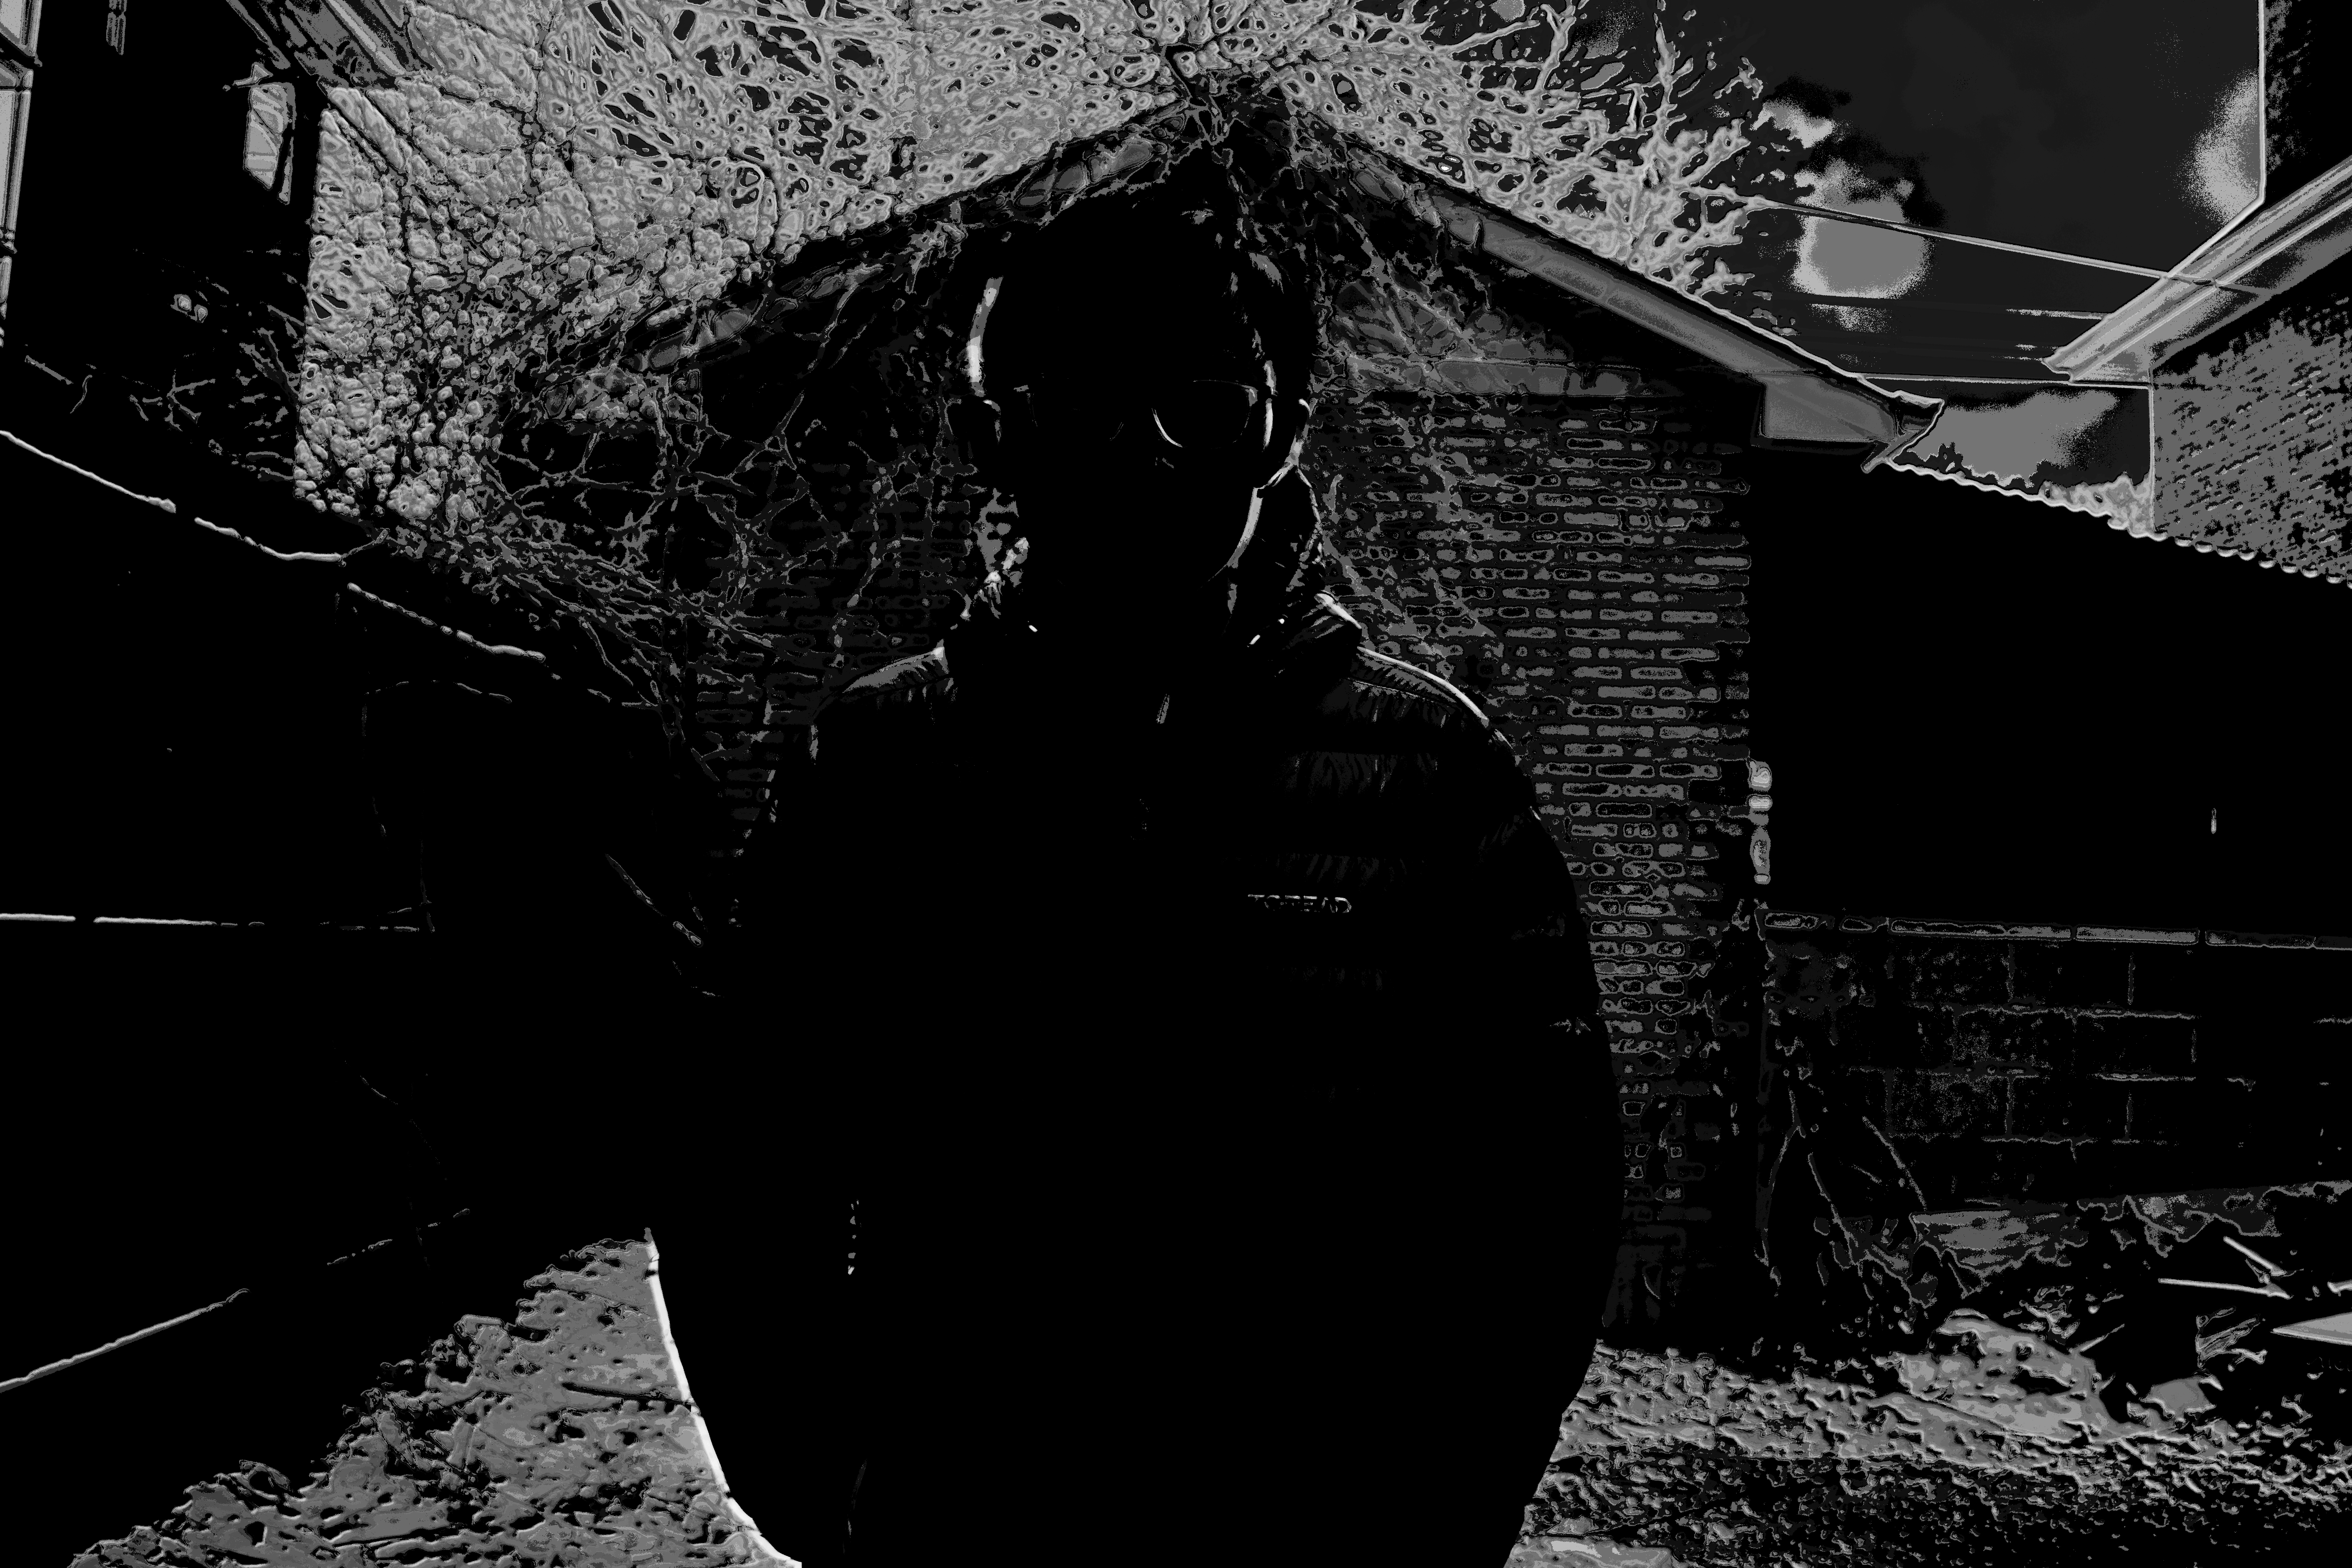
\includegraphics[scale=0.035]{../data/output/arthas_f_ratio.png}
   \caption{flash ratio visualization for flash and no-flash}
\end{figure}
\section{Conclusion}

\begin{figure}[ht]
   \centering
   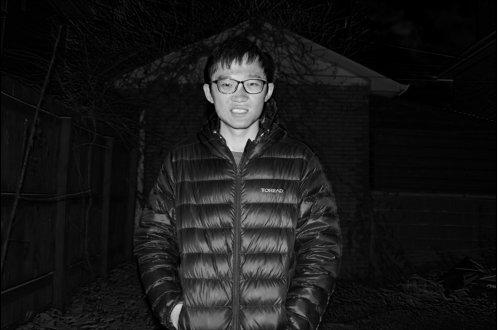
\includegraphics[scale=0.5]{../data/output/Arthas_I_diff.png}
   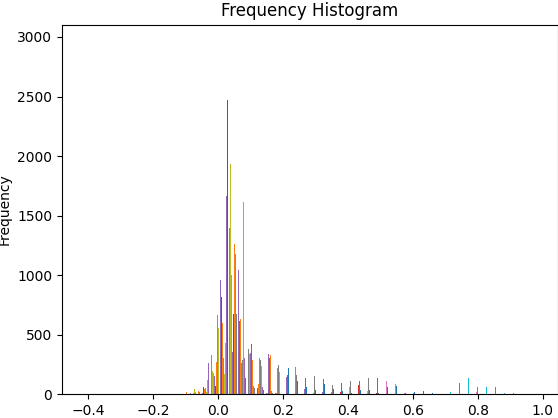
\includegraphics[scale=0.5]{../data/output/idiff_distribution.png}
   \caption{$I_d$ visualization and distribution}
\end{figure}

\begin{figure}[ht]
   \centering
   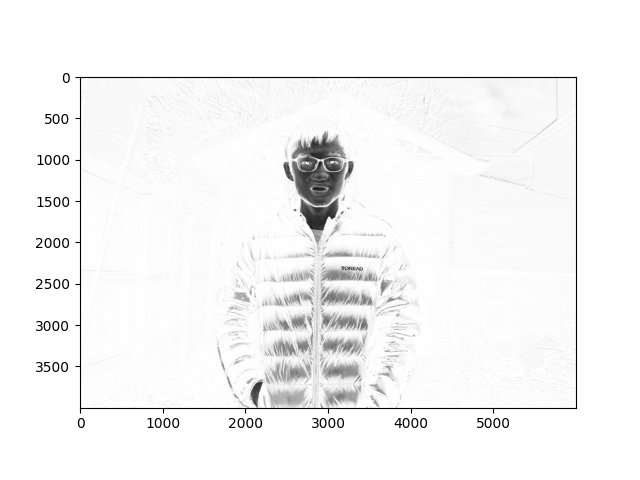
\includegraphics[scale=0.5]{../data/output/p.png}
   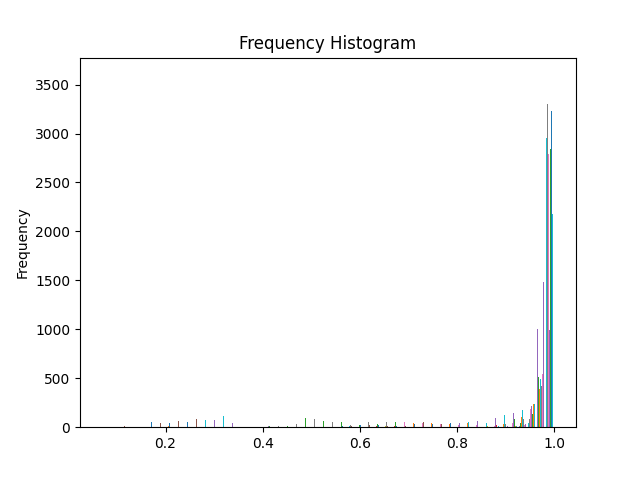
\includegraphics[scale=0.5]{../data/output/p_distr.png}
   \caption{$p_b(x_p)$ visualization and distribution}
\end{figure}

\begin{figure}[ht]
   \centering
   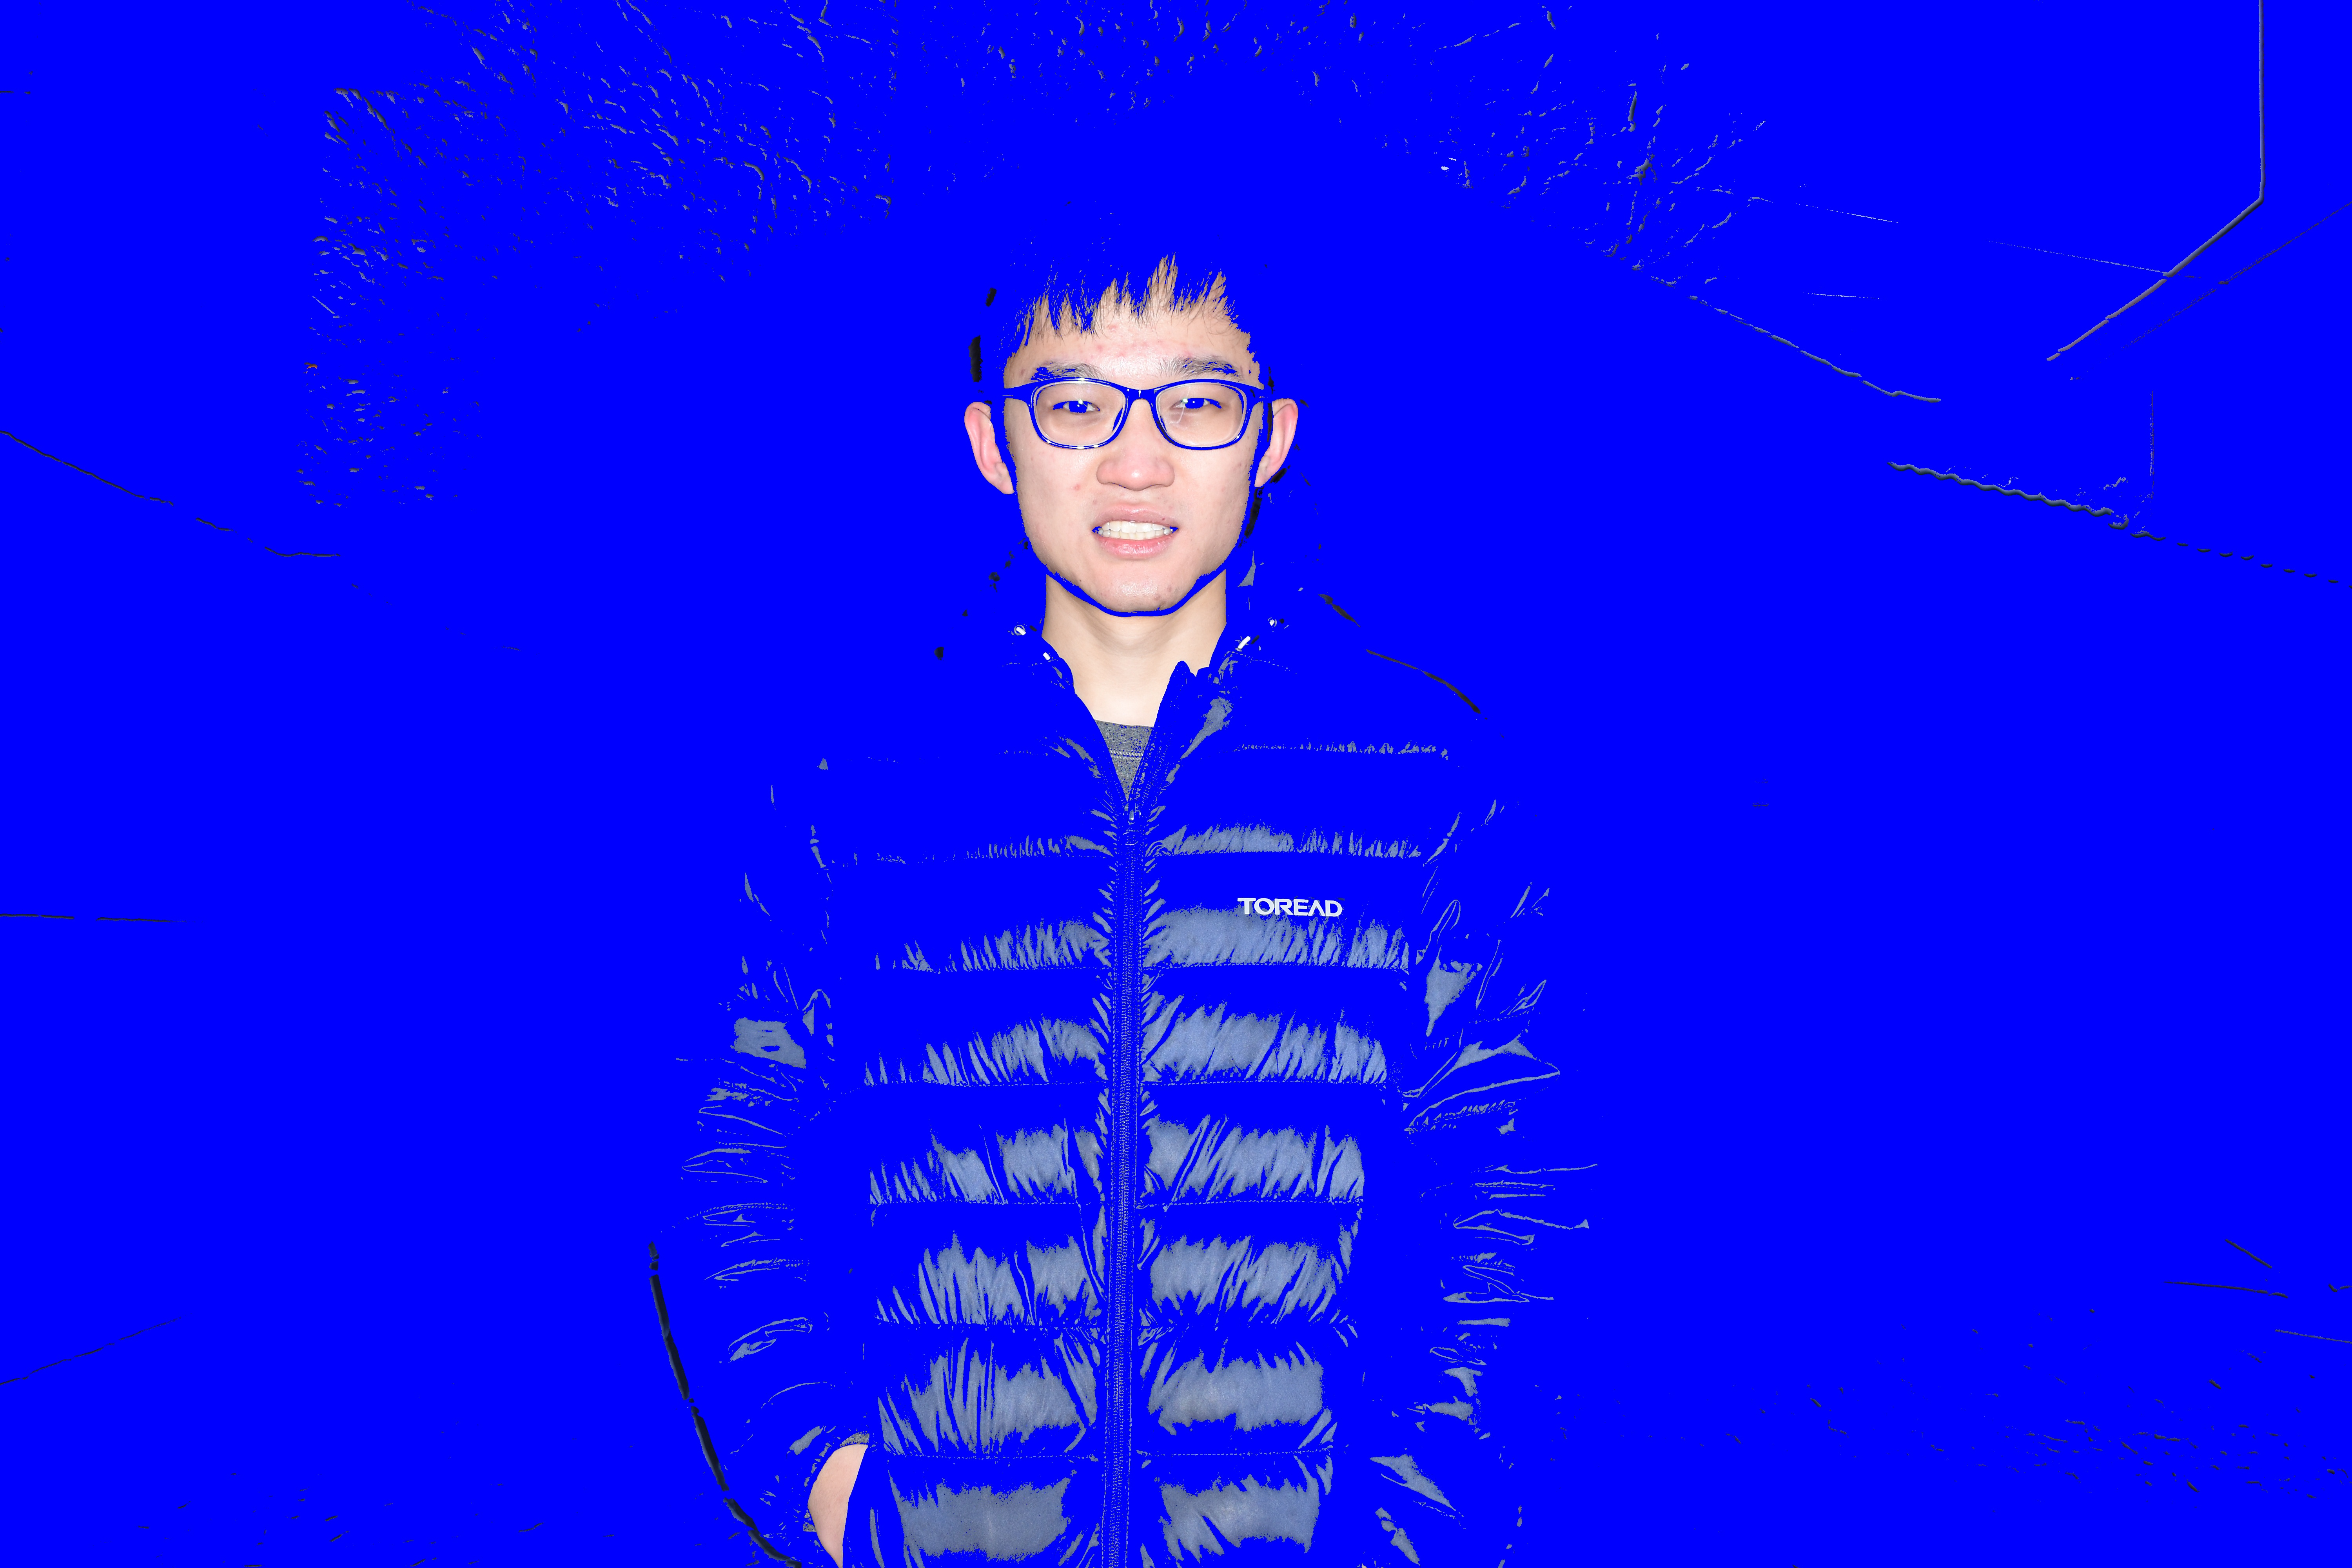
\includegraphics[scale=0.035]{../data/output/arthas_final_f_1.2_0.10_10_10.JPG}
   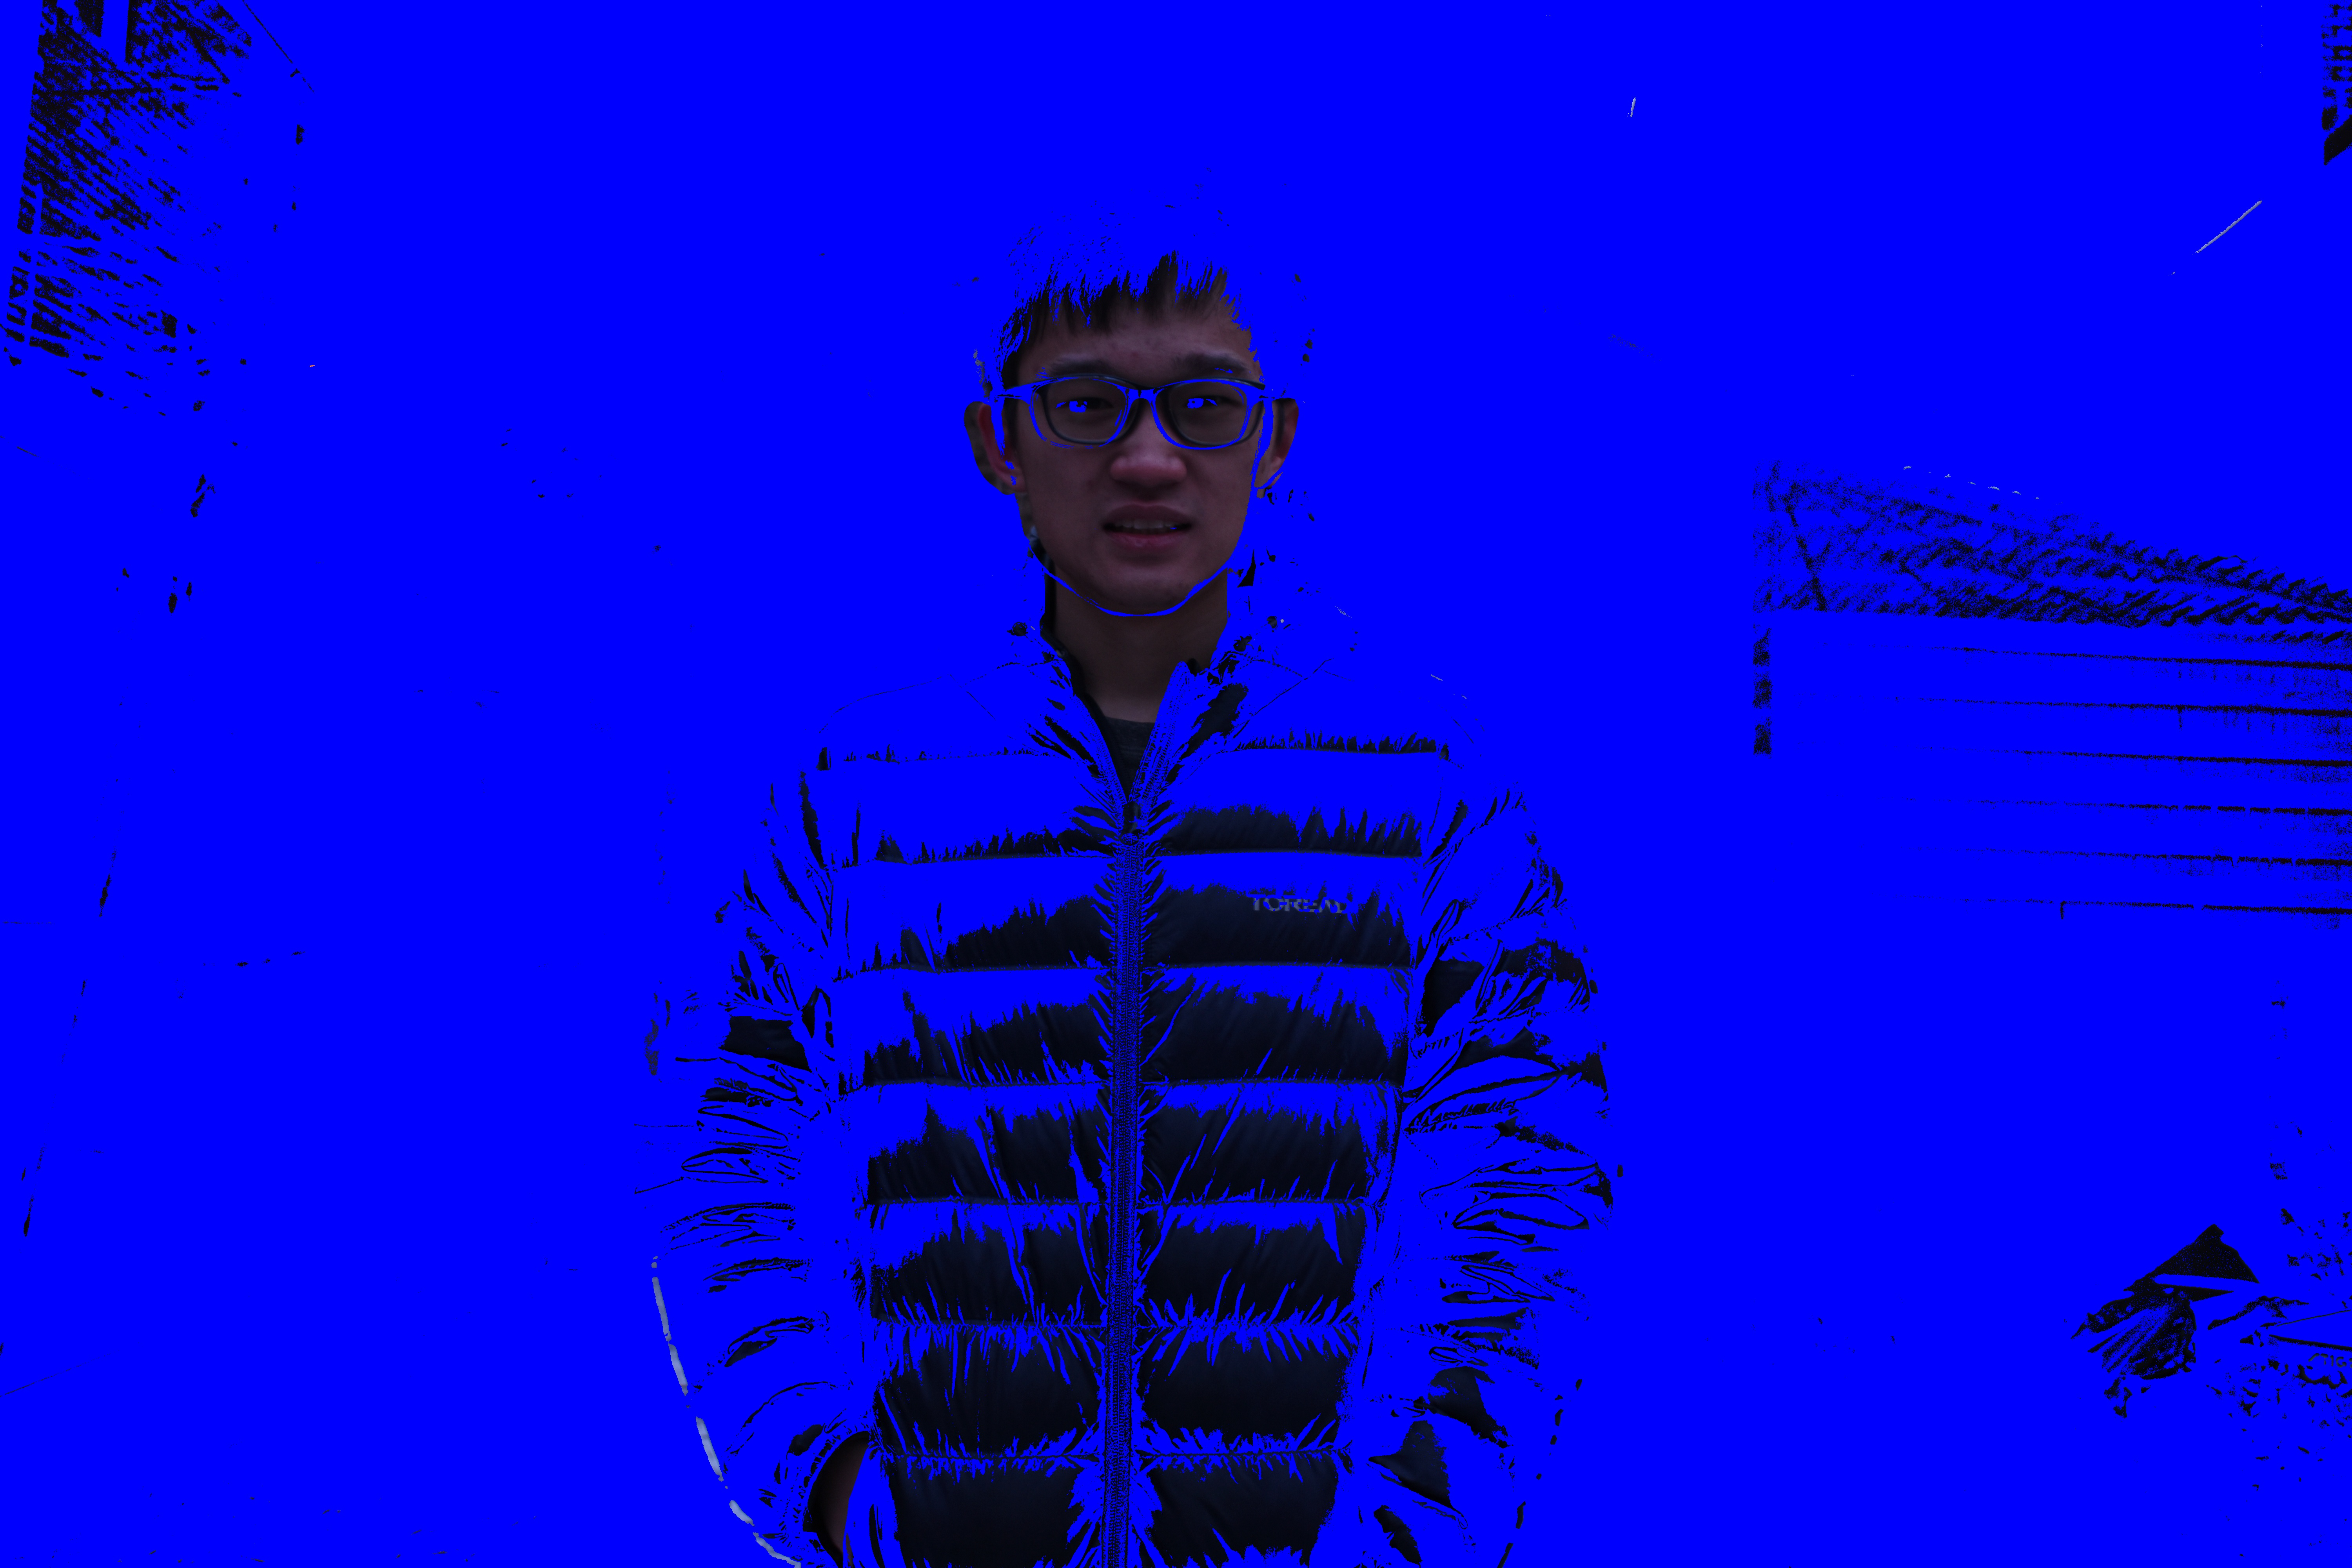
\includegraphics[scale=0.035]{../data/output/arthas_final_nf_1.2_0.10_10_10.JPG}
   \caption{$p_b(x_p)$ visualization and distribution}
\end{figure}

\newpage
\section{Conclusion}

\subsection{Acknowledgement}

%-------------------------------------------------------------------------
\subsection{Illustrations, graphs, and photographs}
{\small\begin{verbatim}
   \usepackage[dvips]{graphicx} ...
   \includegraphics[width=0.8\linewidth]
                   {myfile.eps}
\end{verbatim}
}

{\small
\bibliographystyle{ieee_fullname}
\bibliography{egbib}
}

\end{document}
